\section{Results}
The program was configured to generate a dataset of one million games of Blackjack. This number was chosen, because adding more 0\textquotesingle s to this number increases the time it takes to generate and refine the data set a lot. With one million it took my laptop approximately 5 minutes to generate and 1 minute to refine the data. I could wait longer for more data, but it is not expected to make a difference in the results. one million should be enough data to minimize the coincidence and give reliable results. \\
 \\
Figure 1 and table 1 show all hand values considered difficult with the total number of occurrences when
\begin{itemize}
    \item The player decided to draw 
    \item The player decided to pass
    \item The player decided to draw and won
    \item the player decided to pass and won 
\end{itemize}
An interesting trend appears in the graph with this data. You can see that, the higher the hand value, the less successful it is to draw a card (Blue in figure 1). So drawing a card with a hand value of 12 is more successful than drawing a card at a hand value of 17. This makes sense, because a lower hand value can draw more different cards without going over 21, so has a higher probability of winning.
The same happens to the passing card results, but in opposite order. The higher the hand value, the higher the probability passing will be successful (Red in figure 1). The interesting part in this graph is the differences between these two trends. For the outer two columns the results are very clear:
\begin{itemize}
    \item 12: Probability to win much better by drawing
    \item 13: Probability to win better by drawing
    \item 16: Probability to win better by passing
    \item 17: Probability to win way, way better by passing 
\end{itemize}
In the middle of the graph is the most important data. As expected are 14 and 15 the most difficult hands to make a decision for. When you look at the data it is slightly better to draw a card at a value of 14 and to pass at a value of 15. Based on the big dataset, it is safe to say that is also the best move in this situation. Making the right decision won\textquotesingle t make a big difference for your results while playing the game in real life, but if you happen to play one million games with a value of 14 or 15 in your hand, you could increase your win probability.

\begin{table}[H]
    \caption{Results per value}
\begin{tabular}{|l|l|l|l|l|l|l|}
\hline
 & 12 & 13 & 14 & 15 & 16 & 17 \\ \hline
Total times drawn  & 54477 & 54247 & 53520 & 54795 & 53285 & 47020 \\ \hline
Total times passed  & 57280 & 56577 & 56308 & 57379 & 54557 & 55578 \\ \hline
Total wins by drawing  & 18381 & 16983 & 15696 & 15014 & 14040 & 10255 \\ \hline
Total wins by passing  & 16120 & 16029 & 16032 & 16342 & 15660 & 20723 \\ \hline
\end{tabular}
\end{table}
\begin{figure}[H]
  \centering
  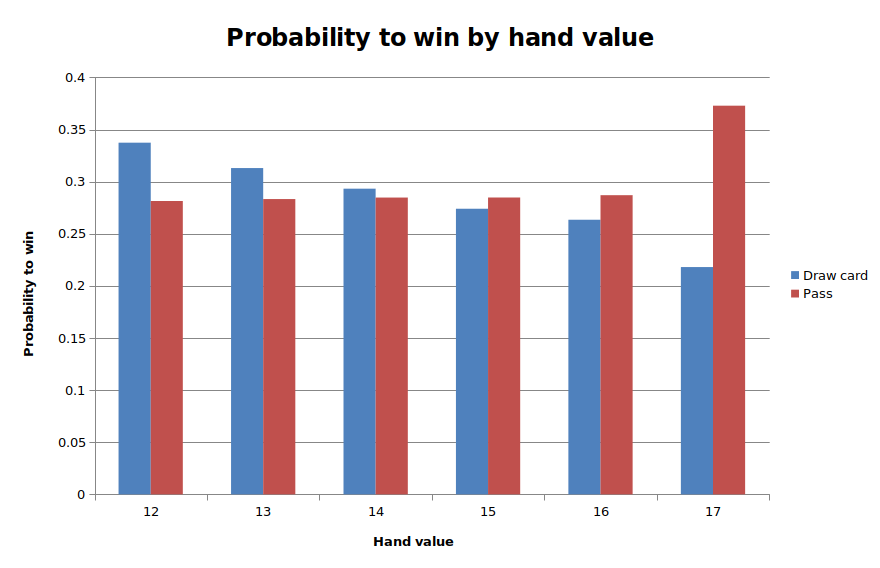
\includegraphics[width=\linewidth]{fig/GraphWinChanceCardValue.png}
  \caption{Graph showing the chance to win for the player by passing and drawing for each hand value in 1000000 games.}
\end{figure}


Figure 2 and table 2 show the total number of occurrences of each possible outcome over the entire experiment of one million games of Blackjack. You can see that the dealer won 513440 / 1000000 * 100 = 51,3 percent of the games, the player won 421942 / 1000000 * 100 = 42,2 percent of the games and only 64618 / 1000000 * 100 = 6,5 percent of the games resulted in a tie. This has a ratio of 1,22 / 1 / 0.15 with Dealer / Player / Tied. This means that, in the long run, the dealer always wins 1,22 times more games than the player. That is 22 percent more games.


\begin{table}[H]
    \caption{Total wins}
\begin{tabular}{|l|l|l|l|}
\hline
 & Dealer & Player & Tied \\ \hline
Total wins &  513440 & 421942 & 64618\\ \hline
\end{tabular}
\end{table}

\begin{figure}[H]
  \centering
  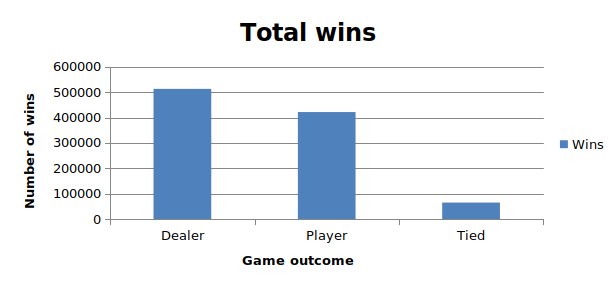
\includegraphics[width=\linewidth]{fig/GraphTotalWins.png}
  \caption{Graph showing total wins for player, dealer and ties in 1000000 games.}
\end{figure} 
